% SOICT 2026 submission --- GAT ablation, v1 tiếng Việt (2026-08-15) --- Springer LNCS format.
% Content = bản dịch tiếng Việt của bản thảo ba-seed đã hoàn thiện:
%   docs/paper/trackA_gat_paper_draft_3seed.md (nguồn số liệu/bảng chuẩn).
% Mọi số liệu, bảng, và kết quả được sao chép nguyên văn từ nguồn tiếng Anh; chỉ nội dung văn bản được dịch.
% Template: llncs.cls từ gói template chính thức SOICT 2026 Springer.
% NOTE: kiểm tra llncs.cls/splncs04.bst với bản tải chính thức SOICT 2026 trước khi nộp cuối cùng.
% Toolchain: pdflatex (inputenc utf8 + babel vietnamese). KHÔNG chạy pdflatex trong quá trình sinh file.
%
\documentclass[runningheads]{llncs}
%
\usepackage[T1]{fontenc}
\usepackage[utf8]{inputenc}
\usepackage[vietnamese]{babel}
\usepackage{graphicx}
\usepackage{amsmath}
\usepackage{amssymb}
\usepackage{booktabs}
%
\begin{document}
%
\title{Dự đoán độ biến động chứng khoán cho thị trường Việt Nam}
%
\titlerunning{Dự đoán độ biến động chứng khoán cho thị trường Việt Nam}
%
% TODO: điền tên và đơn vị tác giả thật trước khi nộp.
\author{Author One\inst{1} \and Author Two\inst{1}}
\authorrunning{Author One et al.}
%
\institute{VNUHCM University of Science, Ho Chi Minh City, Vietnam\\
\email{\{author1,author2\}@student.hcmus.edu.vn}}
%
\maketitle
%
\begin{abstract}
Dự báo độ biến động là cơ sở để thiết lập hạn mức rủi ro, ký quỹ và định giá quyền chọn trên thị
trường chứng khoán Việt Nam. Nghiên cứu này hướng tới dự báo độ biến động cho cổ phiếu Việt Nam nói
chung và sử dụng các cổ phiếu thành phần VN30 (nhóm cổ phiếu thanh khoản cao nhất trên Sở Giao dịch
Chứng khoán TP.\ Hồ Chí Minh) làm nghiên cứu tình huống thực nghiệm. Hai tín hiệu có cấu trúc mà một
mô hình Heterogeneous AutoRegressive (HAR) đơn biến bỏ qua là tin tức tiếng Việt và hiệu ứng lan
truyền chéo giữa các cổ phiếu. Nghiên cứu đề xuất một mô hình đa nhánh song song hợp nhất ba nhánh cho
dự báo phương sai Parkinson đa horizon của một mã cổ phiếu: một LSTM giá theo từng node trên năm đặc
trưng node, một mạng Graph Attention Network (GAT) đa đầu thực sự trên một cạnh dẫn-trễ có hướng khối
lượng-đến-độ biến động (vol$\to$PK), và một LSTM tin tức PhoBERT với cổng theo từng mã. Nhánh GAT tiêu
thụ vector đặc trưng node thô tại gốc dự báo thay vì trạng thái ẩn của LSTM, điều này khớp với ngữ nghĩa
của cạnh (một cú sốc khối lượng của mã nguồn tại $t$ dẫn trước độ biến động của mã đích tại $t{+}1$) và
giữ cho nhánh đồ thị là một góc nhìn cắt ngang độc lập phục vụ một nghiên cứu ablation công bằng. Mô
hình được đánh giá bằng một ablation: từ mô hình đầy đủ, mỗi biến thể được huấn luyện lại bằng cách gỡ
đúng một thành phần (minus\_graph gỡ toàn bộ nhánh GAT, minus\_gate gỡ cổng theo từng mã, minus\_news
gỡ nhánh tin tức), và đóng góp của mỗi thành phần được đo bằng
$\text{effect}(X)=\text{QLIKE}(\text{FULL})-\text{QLIKE}(\text{FULL}{-}X)$ trên tập kiểm tra tách riêng
(held-out), kèm kiểm định Diebold--Mariano để xét ý nghĩa thống kê. HAR cổ điển là baseline tham chiếu.
Qua ba seed và bốn horizon, khác biệt giữa HAR, mô hình đầy đủ, và các biến thể ablation là nhỏ trên
mọi metric. Trên MSE, RMSE, và $R^2$ các giá trị trung bình của các cấu hình nằm trong khoảng 1\% so với
nhau và giá trị tốt nhất luân phiên qua các horizon; trên MAE khác biệt cũng nhỏ tương tự và giá trị
trung bình thấp nhất thay đổi theo horizon. Trên QLIKE, HAR có giá trị trung bình thấp nhất tại h5, h10,
và h22 còn backbone LSTM chỉ-giá có giá trị thấp nhất tại h1. Các kiểm định Diebold--Mariano trên dự báo
seed-ensembled, chạy trên các họ hàm mất mát QLIKE, sai số bình phương, và sai số tuyệt đối, cho thấy
không mô hình nào được ưu tiên trên cả ba. Qua cả năm metric, không cấu hình nào vượt HAR một cách nhất
quán hoặc có ý nghĩa. Đóng góp của bài báo là một quy trình quy đóng góp dựa trên ablation an toàn với
rò rỉ dữ liệu cho một mô hình graph-attention tin tức với hiệu ứng lan truyền có hướng, đối chiếu với một
baseline HAR mạnh trên dữ liệu VN30 hàng ngày thưa.

\keywords{Dự báo độ biến động \and Mạng graph attention \and Hiệu ứng lan truyền có hướng \and Tin tức
tài chính \and PhoBERT \and Thị trường mới nổi.}
\end{abstract}
%
% ======================================================================
\section{Giới thiệu}
\label{sec:intro}
Dự báo độ biến động chi phối các quyết định rủi ro hàng ngày của mọi bộ phận giao dịch cổ phiếu Việt
Nam. Nghiên cứu này giải quyết bài toán dự báo độ biến động cổ phiếu cho thị trường Việt Nam nói chung;
rổ VN30 (khoảng ba mươi cổ phiếu thanh khoản cao nhất trên Sở Giao dịch Chứng khoán TP.\ Hồ Chí Minh)
là nghiên cứu tình huống thực nghiệm được dùng cho tất cả các thí nghiệm vì nó có lịch sử dữ liệu hàng
ngày dài nhất và sạch nhất. Một hệ thống tính ký quỹ định cỡ tài sản đảm bảo từ độ biến động dự báo; một
bộ phận quyền chọn định giá dựa trên đó; một cán bộ quản trị rủi ro thiết lập hạn mức vị thế dựa trên đó.
Các bộ phận VN30 đưa ra những quyết định này trong một môi trường thông tin mà một mô hình dự báo chỉ-giá
bỏ qua: một dòng tin tức tiếng Việt liên tục có thể báo hiệu các cú sốc biến động trước khi chúng đi vào
biên độ giá, và một mạng lưới hiệu ứng lan truyền chéo giữa các cổ phiếu mà một mô hình đơn biến không
thể biểu diễn.

Mô hình HAR cổ điển của Corsi~\cite{corsi2009}, mô hình tuyến tính đơn biến chủ lực hồi quy độ biến động
tương lai trên chính các trung bình hàng ngày, hàng tuần, và hàng tháng của nó, không chấp nhận tín hiệu
nào trong hai tín hiệu trên, và rất khó bị vượt qua~\cite{audrino2025}. Hai mở rộng có cấu trúc có thể
thu hẹp khoảng cách: một kênh tin tức đọc văn bản, và một đồ thị chéo giữa các cổ phiếu cho phép thông
tin của một cổ phiếu đến được cổ phiếu khác. Công trình trước đó trên dự án này đã thiết lập, qua một
phân tích khám phá an toàn với rò rỉ dữ liệu, rằng việc thêm các đặc trưng node cắt ngang (một yếu tố thị
trường và một z-score khối lượng) vượt HAR trên QLIKE, nhưng một cạnh chéo giữa các cổ phiếu \emph{dựa
trên tương quan} không mang lại giá trị ngoài mẫu (out-of-sample) đáng tin cậy vì một yếu tố thị trường
đơn lẻ chi phối sự đồng biến động chéo giữa các cổ phiếu. Điều này thúc đẩy lựa chọn thiết kế trung tâm
của nghiên cứu hiện tại: thay vì một cạnh tương quan đối xứng, nghiên cứu kiểm tra một \textbf{cạnh
dẫn-trễ có hướng khối lượng$\to$độ biến động} --- khối lượng bất thường hôm nay của một mã nguồn liên kết
với độ biến động biên độ ngày mai của một mã đích --- mã hóa một quan hệ dự báo, theo hướng nhân quả mà
một cạnh tương quan đồng thời không thể có.

Nghiên cứu tích hợp cạnh này vào một kiến trúc đa nhánh song song (một nhánh thời gian LSTM, một nhánh
đồ thị GAT, và một nhánh tin tức có cổng, được ghép nối tại một head chung) và định lượng, theo từng
thành phần và từng horizon, đóng góp biên của mỗi phần bằng một ablation: xây dựng mô hình đầy đủ, sau đó
huấn luyện lại một biến thể với đúng một thành phần bị gỡ, và quy đóng góp của mỗi thành phần thành mức
thay đổi QLIKE held-out mà nó gây ra. Bài báo này có ba đóng góp.
\begin{enumerate}
\item \textbf{Một mô hình graph-attention tin tức vol$\to$PK có hướng trên một backbone đa nhánh song
song.} Mô hình hợp nhất một LSTM giá theo từng node, một GAT đa đầu thực sự trên một cạnh dẫn-trễ có
hướng khối lượng-đến-độ biến động, và một nhánh tin tức PhoBERT có cổng. GAT tiêu thụ vector đặc trưng
node thô tại gốc dự báo, điều này khớp với ngữ nghĩa của cạnh và giữ cho nhánh đồ thị là một góc nhìn
cắt ngang độc lập (Mục~\ref{sec:method}).
\item \textbf{Một ablation đối chiếu với một baseline HAR mạnh.} Từ mô hình đầy đủ, mỗi biến thể được
huấn luyện lại theo từng thành phần bị gỡ --- minus\_graph (toàn bộ nhánh GAT), minus\_gate, minus\_news
--- nên mọi hiệu ứng được đo trên cùng một cơ sở, và đóng góp biên của mỗi thành phần được báo cáo là
$\text{effect}(X)=\text{QLIKE}(\text{FULL})-\text{QLIKE}(\text{FULL}{-}X)$ kèm kiểm định
Diebold--Mariano (Mục~\ref{sec:results}).
\item \textbf{Một đánh giá đa horizon an toàn với rò rỉ dữ liệu.} Tất cả mô hình được đánh giá tại các
horizon 1, 5, 10, và 22 ngày giao dịch trên một phân chia theo thời gian với các scaler chỉ dùng dữ liệu
train và một cạnh đông cứng chỉ ước lượng trên train, với tập kiểm tra held-out là kết quả báo cáo, qua
ba seed cùng các kiểm định ý nghĩa trên dự báo seed-ensembled (Mục~\ref{sec:setup}
và~\ref{sec:results}).
\end{enumerate}

% ======================================================================
\section{Công trình liên quan}
\label{sec:related}
Chúng tôi phân nhóm công trình trước thành bốn họ và nêu vị trí của mô hình đề xuất so với từng họ.

\subsubsection{Mô hình độ biến động kinh tế lượng.}
Mô hình HAR~\cite{corsi2009} và các đầu vào dựa trên biên độ của nó~\cite{parkinson1980} đặt ra tiêu
chuẩn cho dự báo độ biến động hàng ngày và vẫn khó bị vượt qua. HAR hồi quy độ biến động tương lai trên
các trung bình trượt hàng ngày, hàng tuần, và hàng tháng, xấp xỉ tính nhớ dài của độ biến động bằng một
hồi quy tuyến tính tiết kiệm. Mở rộng HARQ~\cite{bpq2016} thu nhỏ hệ số hàng ngày khi ước lượng độ biến
động nhiễu. Một nghiên cứu có kiểm soát quy mô lớn cho thấy các mô hình học máy đã được tinh chỉnh không
vượt được một HAR được tái ước lượng cẩn thận trên QLIKE và MSE khi cả hai dùng cùng tập
thông tin~\cite{audrino2025}. Các mô hình này là đơn biến và tuyến tính: không kênh nào chấp nhận văn
bản, và không kênh nào ghép nối một cổ phiếu với cổ phiếu khác. Chúng tôi giữ ba thang HAR trong số các
đặc trưng node và thêm các kênh tin tức và chéo giữa các cổ phiếu có hướng mà HAR bỏ qua; HAR cổ điển là
baseline mà mọi thành phần phải vượt qua.

\subsubsection{Bộ dự báo sâu và dựa trên đồ thị.}
Các bộ dự báo LSTM~\cite{hochreiter1997} nắm bắt cấu trúc thời gian phi tuyến, và các mạng graph
attention~\cite{velickovic2018} mô hình hóa sự ghép nối chéo giữa các tài sản; các thiết kế lai LSTM-GNN
kết hợp cả hai~\cite{sonani2025}. Chen và Robert~\cite{chen2022} dự báo độ biến động thực hiện đa biến
với một đồ thị trên khoảng 500 mã S\&P. Liên quan nhất, Zhang, Pu, Cucuringu và
Dong~\cite{zhang2025gnnhar} xây dựng một graph-neural-network HAR (GNNHAR) trên DJIA-30 và, dưới một
Model Confidence Set, phát hiện rằng hiệu ứng lan truyền đồ thị chéo giữa các cổ phiếu đa bước không mang
lại lợi thế rõ ràng: các mức tăng đến từ việc mô hình hóa tính phi tuyến và từ việc chuyển hàm mất mát
huấn luyện từ MSE sang QLIKE. Kết quả null có kiểm soát của họ trên thành phần đồ thị thúc đẩy việc chúng
tôi chuyển từ một cạnh tương quan đối xứng sang một cạnh dẫn-trễ có hướng, được kiểm tra tại đây dưới một
ablation.

\subsubsection{Đồ thị hiệu ứng lan truyền có hướng và dẫn-trễ.}
Một cạnh tương quan đối xứng trộn lẫn sự đồng biến động đồng thời (phần lớn là một yếu tố thị trường) với
cấu trúc dự báo. Các thước đo hiệu ứng lan truyền có hướng --- ví dụ các chỉ số hiệu ứng lan truyền độ
biến động~\cite{diebold2012} --- mã hóa ai-dẫn-ai và bất đối xứng theo cấu tạo. Chúng tôi hiện thực hóa
một cạnh có hướng từ khối lượng bất thường của một mã nguồn đến độ biến động biên độ ngày kế tiếp của một
mã đích, dựa trên quan hệ dẫn-trễ khối lượng--độ biến động, và đông cứng nó trên cửa sổ huấn luyện.

\subsubsection{Dự báo tăng cường bằng tin tức và văn bản.}
Các bộ dự báo tăng cường văn bản thêm điểm cảm xúc hoặc embedding tin tức~\cite{ouyang2021,das2024},
thường hợp nhất một tín hiệu toàn thị trường đơn lẻ bằng ghép nối trên các thị trường tiếng Anh hoặc
tiếng Trung. Chúng tôi làm việc bằng tiếng Việt với PhoBERT~\cite{phobert2020} trên VN30 và thêm một cổng
theo từng mã cho phép một lượng tin tức khác nhau cho mỗi cổ phiếu.

% ======================================================================
\section{Dữ liệu}
\label{sec:data}

\subsubsection{Vũ trụ dữ liệu (nghiên cứu tình huống).}
Phương pháp hướng tới thị trường chứng khoán Việt Nam nói chung; VN30 là vũ trụ nghiên cứu tình huống
cho các thí nghiệm. Chúng tôi dùng 33 cổ phiếu thành phần VN30 với dữ liệu open-high-low-close-volume
(OHLCV) hàng ngày. Độ dài chuỗi trải từ khoảng 1.300 phiên (SSB, niêm yết 2021) đến khoảng 4.900 (VNM,
ACB, từ 2006). Vũ trụ là một tập cố định theo thời điểm kiểu VN30 chứ không phải chỉ số động, một hạn chế
được nêu trong mục Hạn chế.

\subsubsection{Mục tiêu dự báo.}
Chúng tôi dự báo độ biến động biên độ Parkinson hàng ngày tại các horizon 1, 5, 10, và 22 ngày giao dịch
phía trước: mục tiêu là giá trị của estimator ở một ngày đơn lẻ tại ngày $t{+}h$ (tức $\text{PK}(t{+}h)$),
không phải trung bình trên $h$ ngày kế tiếp. Estimator Parkinson dùng giá cao nhất $H$ và thấp nhất $L$
trong ngày:
\begin{equation}
\sigma^2_{\text{Park}} = \frac{\left(\ln(H/L)\right)^2}{4\ln 2}.
\label{eq:parkinson}
\end{equation}
Cột \texttt{parkinson\_volatility} đã xử lý về mặt số học là estimator \textbf{phương sai} Parkinson
($\sigma^2$, không âm), và mọi mô hình trong bài báo này dự báo cùng đại lượng phương sai thực hiện hàng
ngày này.

\subsubsection{Đặc trưng node.}
Mỗi ticker-day mang năm đặc trưng node theo một thứ tự cố định, tất cả với các cửa sổ 22 ngày giao dịch
thống nhất để khớp với thang HAR hàng tháng:
\begin{enumerate}
\item \texttt{pk\_daily} --- phương sai Parkinson tại $t$, được cắt về $\pm 3\sigma$ dùng thống kê train.
\item \texttt{har\_weekly} --- trung bình 5 ngày lùi của \texttt{pk\_daily}.
\item \texttt{har\_monthly} --- trung bình 22 ngày lùi của \texttt{pk\_daily}.
\item \texttt{market\_pk} --- trung vị cắt ngang của $\sqrt{\text{PK}}$ qua các mã hiện diện tại $t$ (một
yếu tố thị trường đồng thời; chỉ dùng cột $t$).
\item \texttt{volume\_zscore} --- z-score trượt-22 lùi của $\log(1+\text{volume})$; các mã không có chuỗi
khối lượng OHLCV nhận giá trị trung tính 0.0.
\end{enumerate}

\subsubsection{Bảng tin tức.}
Mỗi bài báo tiếng Việt (tiêu đề và đoạn dẫn) đi qua PhoBERT~\cite{phobert2020} một lần, tạo ra một
embedding 768 chiều được giảm bằng PCA (khớp trước mốc cắt huấn luyện) thành một vector theo từng ngày
theo từng cổ phiếu gồm 146 chiều (các thành phần embedding, các chuẩn theo nhóm, các trung bình có trọng
số mũ với chu kỳ bán rã 30 ngày giao dịch, và số đếm chủ đề). Tin tức thiếu vào một ngày là một vector
không với bit mask đặt bằng không, và một cửa sổ hoàn toàn thiếu vẫn tạo ra một biểu diễn hữu hạn.

\subsubsection{Cạnh vol$\to$PK có hướng.}
Ma trận kề là có hướng: với mỗi mã đích $j$, chúng tôi kết nối Top-5 mã nguồn $i$ được xếp hạng theo
tương quan dẫn-trễ chỉ ước lượng trên train
$\text{corr}(\text{volume\_shock}_i(t),\ \sqrt{\text{PK}_j}(t{+}1))$. Các cạnh được ước lượng chỉ trên
các hàng train và đông cứng cho validation và test (an toàn với rò rỉ dữ liệu), và các self-loop được
giữ trên đường chéo.

\subsubsection{Phân chia theo thời gian và kiểm soát rò rỉ dữ liệu.}
Chuỗi của mỗi mã được chia theo thời gian thành 70\% train, 15\% validation, và 15\% test trước khi sinh
đặc trưng, khớp scaler, hoặc xây cửa sổ; các chuỗi sớm nhất bắt đầu năm 2006. Phân chia được áp dụng theo
từng mã trên dòng thời gian riêng của nó, nên các ranh giới lịch train/validation/test khác nhau giữa các
mã --- một mã niêm yết năm 2021 có các ranh giới muộn hơn một mã giao dịch từ 2006 --- đó chính là lý do
một bảng đồng bộ node cố định sẽ sụp đổ và tại sao phân chia gộp theo từng mã được dùng. Các scaler giá
và mục tiêu theo từng mã được khớp chỉ trên phần train và được chọn khi đánh giá bằng \texttt{ticker\_id}
tường minh. Một đặc trưng tin tức cho một mẫu chỉ dùng thông tin có sẵn tính đến gốc dự báo của mẫu đó.
Đánh giá đọc các mục tiêu thô đã lưu thay vì nghịch đảo biến đổi một mục tiêu chuẩn hóa đã bị cắt. Trên
bảng dữ liệu gộp có mask, các tập đánh giá giữ, tại horizon năm ngày, 14.418 quan sát validation và
14.464 quan sát test node hiện diện, được chia sẻ giống hệt qua mọi bậc; số lượng thay đổi nhẹ theo
horizon (ví dụ 14.550/14.596 tại h1 và 14.253/14.299 tại h10) vì dịch chuyển mục tiêu làm thay đổi số cửa
sổ đủ điều kiện.

% ======================================================================
\section{Phương pháp}
\label{sec:method}
Chúng tôi mô tả mô hình đầy đủ đề xuất trước, sau đó định nghĩa các biến thể ablation là các thao tác gỡ
thành phần khỏi nó. Mô hình dự báo phương sai Parkinson $h$-ngày-tới của một mã từ bốn đầu vào: một cửa
sổ giá 22 ngày của năm đặc trưng node, một cửa sổ tin tức 22 ngày của các đặc trưng PhoBERT với một mask,
danh tính của mã, và ma trận kề vol$\to$PK có hướng trên các mã hiện diện cùng ngày.

\begin{figure}[t]
\centering
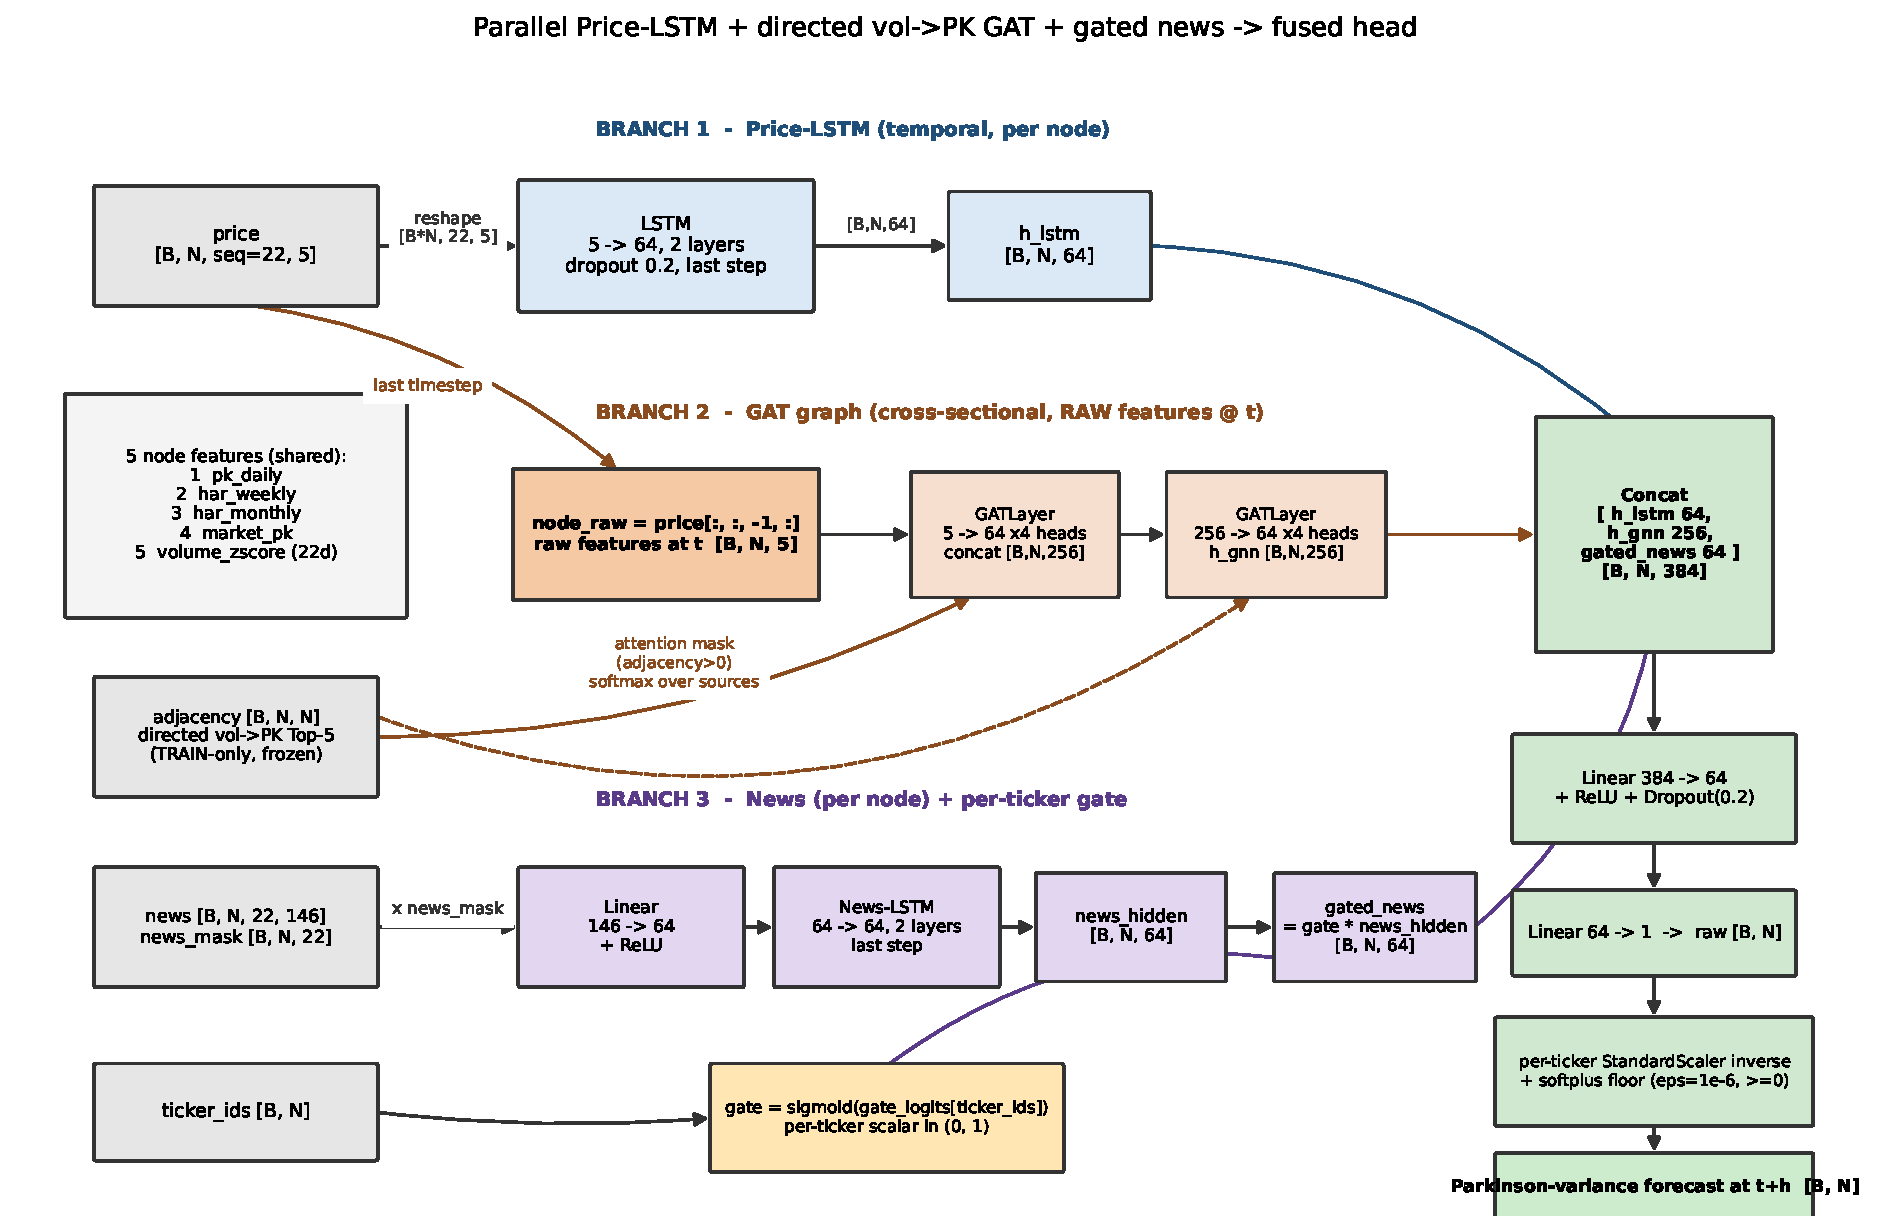
\includegraphics[width=\textwidth]{diagrams/trackA_gat_architecture.pdf}
\caption{Kiến trúc mô hình: các nhánh song song LSTM-giá, GAT vol$\to$PK có hướng (trên đặc trưng node
thô), và nhánh tin tức PhoBERT có cổng, được ghép nối vào một head với một sàn dương softplus.}
\label{fig:arch}
\end{figure}

\subsubsection{Mô hình đầy đủ đề xuất.}
Ba nhánh chạy song song và ghép nối tại một head chung.
\begin{itemize}
\item \textbf{(i) Nhánh Price-LSTM (thời gian, theo từng node).} Một LSTM hai lớp (kích thước ẩn 64,
dropout 0.2) đọc cửa sổ 22 ngày của năm đặc trưng node của mỗi mã thành một biểu diễn giá
$h_{\text{lstm}}$ ($\mathbb{R}^{64}$ mỗi node).
\item \textbf{(ii) Nhánh đồ thị GAT (cắt ngang).} Đầu vào node là vector đặc trưng node \textbf{thô} tại
bước thời gian cuối, $\text{node\_raw}=\text{price}[:, :, {-}1, :]\in\mathbb{R}^{5}$, không phải trạng
thái ẩn của LSTM. Hai lớp GAT đa đầu tự viết ($5\to256$, rồi $256\to256$; 4 đầu) với attention được mask
bởi ma trận kề (softmax trên các node nguồn, đầu ra ELU) tạo ra $h_{\text{gnn}}\in\mathbb{R}^{256}$. Việc
tiêu thụ các đặc trưng thô khớp với ngữ nghĩa của cạnh (\texttt{volume\_shock} trực tiếp có sẵn cho
attention) và giữ cho nhánh đồ thị độc lập với nhánh LSTM, nên gỡ nó là một ablation sạch. Khi đồ thị bị
tắt, ma trận kề là ma trận đơn vị (chỉ self-loop).
\item \textbf{(iii) Nhánh tin tức với cổng theo từng mã.} Vector tin tức hàng ngày 146 chiều đi qua một
phép chiếu tuyến-tính-cộng-ReLU vào một LSTM hai lớp (kích thước ẩn 64) trên cửa sổ có mask, tạo ra một
biểu diễn tin tức, được nhân tỷ lệ bởi một cổng sigmoid theo từng mã đã học,
\begin{equation}
\text{news}^{\text{gated}}_{i} = \sigma(g_i)\cdot \text{news}_{i}, \qquad i=1,\dots,N.
\label{eq:gate}
\end{equation}
\end{itemize}
Head ghép nối $[h_{\text{lstm}}(64),\ h_{\text{gnn}}(256),\ \text{news}^{\text{gated}}(64)]$
($\mathbb{R}^{384}$) và ánh xạ nó qua một stack tuyến-tính-ReLU-dropout-tuyến-tính đến dự báo. Một
\textbf{sàn dương} softplus ($\varepsilon=10^{-6}$, áp dụng trong không gian đã khử chuẩn hóa và giống hệt
qua mọi bậc so sánh) kẹp các dự báo tránh xa phương sai không dương trước QLIKE.

\begin{figure}[t]
\centering
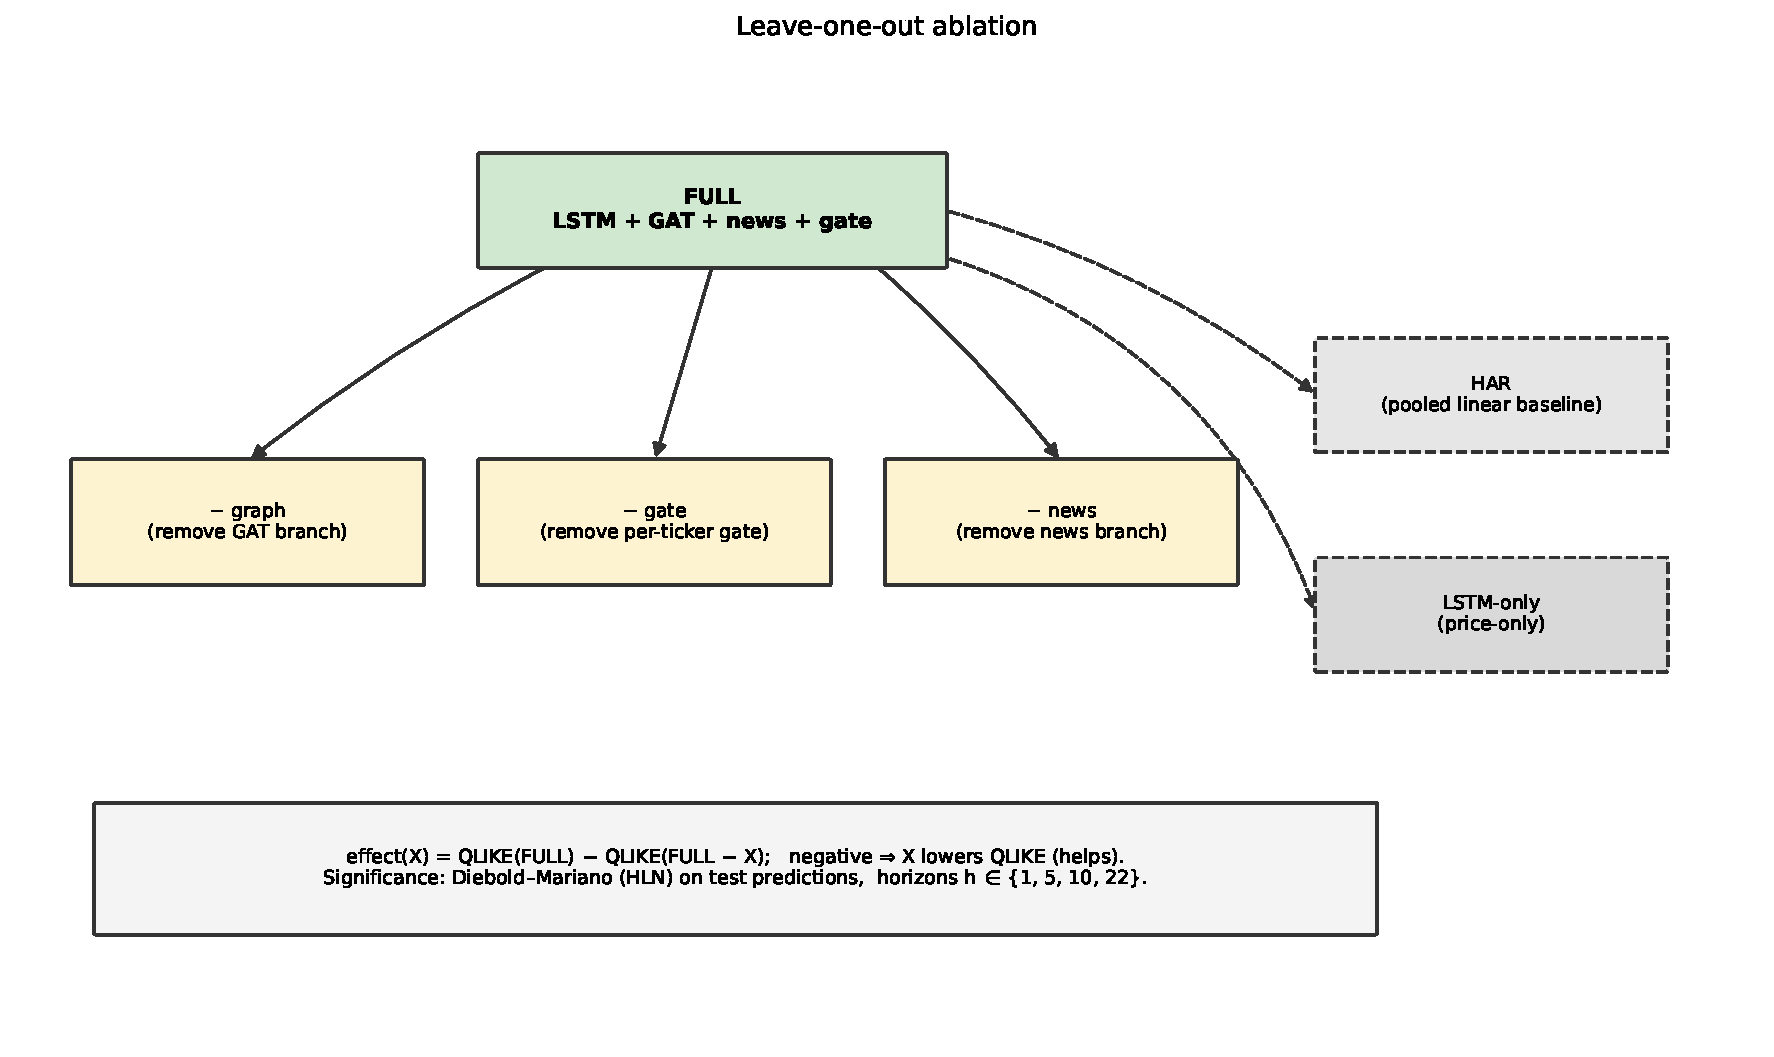
\includegraphics[width=\textwidth]{diagrams/trackA_gat_ablation.pdf}
\caption{Ablation: từ FULL, mỗi biến thể gỡ một thành phần ($-$graph, $-$gate, $-$news); HAR và một mô
hình LSTM-only chỉ-giá là các baseline tham chiếu.
$\text{effect}(X)=\text{QLIKE}(\text{FULL})-\text{QLIKE}(\text{FULL}{-}X)$.}
\label{fig:ablation}
\end{figure}

\subsubsection{Các biến thể ablation.}
Chúng tôi xây mô hình đầy đủ, sau đó huấn luyện lại một biến thể theo từng thành phần bị gỡ, nên mọi hiệu
ứng được đo trên cùng một cơ sở (mỗi biến thể huấn luyện trong cùng chế độ đồ thị bật/tắt mà nó được đánh
giá --- không có sự lệch train/eval):
\begin{itemize}
\item \textbf{FULL} --- LSTM + đồ thị GAT vol$\to$PK có hướng + tin tức + cổng theo từng mã.
\item \textbf{minus\_graph} --- FULL với \textbf{toàn bộ nhánh GAT bị gỡ} (không xây node/cạnh/GAT; head
lấy $[h_{\text{lstm}},\ \text{news}^{\text{gated}}]\in\mathbb{R}^{128}$). Điều này cô lập toàn bộ hệ
thống con đồ thị, không chỉ các cạnh.
\item \textbf{minus\_gate} --- FULL không có cổng theo từng mã.
\item \textbf{minus\_news} --- FULL không có nhánh tin tức (cổng là một no-op khi không có tin tức).
\item \textbf{HAR} --- một hồi quy tuyến tính HAR gộp theo từng mã trên ba thang HAR; sàn mà mọi thành
phần phải vượt qua.
\end{itemize}
Đóng góp của thành phần $X$ là
$\text{effect}(X)=\text{QLIKE}(\text{FULL})-\text{QLIKE}(\text{FULL}{-}X)$ trên tập kiểm tra held-out;
một giá trị âm nghĩa là gỡ $X$ làm tăng QLIKE, tức $X$ có ích.

\subsubsection{Huấn luyện.}
Các mô hình sâu dùng Adam (tốc độ học $10^{-3}$), weight decay $10^{-5}$, dropout 0.2, và cắt gradient
tại 1.0, với việc chọn checkpoint tốt nhất trên validation. Vì các mô hình gộp hội tụ trong vài epoch rồi
overfit, huấn luyện dùng early stopping (patience 3, tối thiểu 6 epoch) dưới một trần 12 epoch. Mọi cấu
hình được huấn luyện dưới ba seed (42, 123, 2026); các metric test được báo cáo là mean(std) qua ba seed,
và các kiểm định Diebold--Mariano chạy trên các dự báo test seed-ensembled.

% ======================================================================
\section{Thiết lập thực nghiệm}
\label{sec:setup}

\subsubsection{Các metric.}
Mọi cấu hình báo cáo năm metric trên thang phương sai thô: MSE, RMSE, MAE, $R^2$, và QLIKE. QLIKE, hàm
mất mát tựa-hợp-lý (quasi-likelihood) chuẩn trong tài liệu độ biến động thực hiện~\cite{patton2011}, phạt
việc dự báo thiếu nặng hơn dự báo thừa và chịu được nhiễu trong proxy độ biến động:
\begin{equation}
\text{QLIKE} = \frac{1}{T}\sum_{t=1}^{T}\left(\frac{\hat{\sigma}^2_t}{\sigma^2_t}
 - \ln\frac{\hat{\sigma}^2_t}{\sigma^2_t} - 1\right).
\label{eq:qlike}
\end{equation}
Độ chính xác định hướng không được báo cáo; mục Hạn chế nêu lý do nó không mang thông tin cho mục tiêu
này.

\subsubsection{Hàm mục tiêu huấn luyện.}
Tất cả cấu hình sâu tối thiểu hóa sai số bình phương trung bình giữa đầu ra mô hình và mục tiêu chuẩn hóa
theo từng mã; QLIKE và các metric khác chỉ được tính khi đánh giá, sau khi nghịch đảo chuẩn hóa về thang
phương sai thô, nên hàm mất mát QLIKE tỷ lệ không bao giờ đi vào gradient.

\subsubsection{Giao thức báo cáo.}
Việc chọn mô hình (early-stopping, best-checkpoint) chỉ dùng phân chia validation; tất cả kết quả báo cáo
và kiểm định ý nghĩa được tính trên tập kiểm tra held-out; validation chỉ được dùng để chọn mô hình, và
không có metric validation nào được báo cáo.

\subsubsection{Ý nghĩa thống kê.}
Chúng tôi bổ sung so sánh metric bằng một kiểm định Diebold--Mariano (DM) trên chuỗi mất mát QLIKE (và
sai số bình phương) theo từng quan sát (độ trễ cắt HAC $h{-}1$, hiệu chỉnh Harvey--Leybourne--Newbold),
kiểm tra tính bằng nhau về độ chính xác dự báo trực tiếp trên các quan sát held-out. Kiểm định DM chạy
trên các dự báo seed-ensembled (dự báo trung bình theo từng quan sát qua các seed 42, 123, 2026).

\subsubsection{Hiện thực và tính toán.}
Tất cả mô hình được hiện thực bằng PyTorch (lớp GAT tự viết; không dùng thư viện đồ thị bên ngoài) và
dùng một GPU CUDA. Các lần chạy dùng một GPU NVIDIA GeForce RTX~4060 Laptop dưới PyTorch~2.6 với
CUDA~12.4.

% ======================================================================
\section{Kết quả}
\label{sec:results}

\subsection{Các metric test held-out qua các horizon}
\label{sec:metrics}
Bảng~\ref{tab:metrics} báo cáo cả năm metric qua bốn horizon, mean(std) qua ba seed. Đọc qua các horizon:
trên các metric sai số bình phương (MSE, RMSE, $R^2$), các giá trị trung bình của các cấu hình nằm trong
khoảng 1\% so với nhau và hàng tốt nhất luân phiên (minus\_news tại h1, minus\_gate/LSTM-only tại h5/h10,
HAR tại h22); trên MAE khác biệt cũng nhỏ tương tự và giá trị trung bình thấp nhất thay đổi theo horizon
(LSTM-only tại h1, bốn cấu hình gần bằng nhau quanh 5.97 tại h5, FULL tại h10, minus\_graph tại h22);
trên QLIKE, HAR có giá trị trung bình thấp nhất tại h5, h10, và h22 còn LSTM-only chỉ-giá có giá trị
trung bình thấp nhất tại h1. Các độ lệch chuẩn báo cáo là nhỏ so với khoảng cách giữa các cấu hình ngoại
trừ tại h10, nơi các giá trị trung bình QLIKE của FULL và minus\_news mang độ phân tán seed lớn hơn (std
0.034 và 0.053).

\begin{table}[t]
\caption{Các metric TEST held-out theo horizon, mean(std) qua ba seed (42, 123, 2026). Thấp hơn là tốt
hơn cho MSE, RMSE, MAE, QLIKE; cao hơn cho $R^2$. In đậm đánh dấu giá trị trung bình tốt nhất mỗi cột
trong từng horizon; cùng các quan sát test được chia sẻ qua mọi hàng của một horizon. HAR là một hồi quy
tuyến tính xác định (std 0.00).}
\label{tab:metrics}
\centering
\begin{tabular}{lccccc}
\toprule
Config & MSE ($\times10^{-6}$) $\downarrow$ & RMSE ($\times10^{-3}$) $\downarrow$ & MAE ($\times10^{-4}$) $\downarrow$ & $R^2$ $\uparrow$ & QLIKE $\downarrow$ \\
\midrule
\multicolumn{6}{l}{\textit{h = 1 ngày giao dịch}}\\
HAR         & 4.05 (0.00) & 2.014 (0.000) & 5.41 (0.00) & 0.8192 (0.0000) & 0.4813 (0.0000) \\
FULL        & 4.06 (0.08) & 2.015 (0.020) & 5.45 (0.07) & 0.8189 (0.0036) & 0.4853 (0.0059) \\
minus\_graph & 4.04 (0.05) & 2.009 (0.012) & 5.41 (0.05) & 0.8200 (0.0022) & 0.4797 (0.0045) \\
minus\_gate  & 4.02 (0.10) & 2.006 (0.025) & 5.42 (0.06) & 0.8206 (0.0045) & 0.4830 (0.0070) \\
minus\_news  & \textbf{4.01 (0.08)} & \textbf{2.003 (0.021)} & 5.42 (0.06) & \textbf{0.8210 (0.0037)} & 0.4824 (0.0071) \\
LSTM-only   & 4.08 (0.09) & 2.021 (0.022) & \textbf{5.36 (0.05)} & 0.8179 (0.0040) & \textbf{0.4791 (0.0051)} \\
\midrule
\multicolumn{6}{l}{\textit{h = 5 ngày giao dịch}}\\
HAR         & 5.23 (0.00) & 2.287 (0.000) & 6.05 (0.00) & 0.7672 (0.0000) & \textbf{0.5735 (0.0000)} \\
FULL        & 5.19 (0.08) & 2.278 (0.018) & \textbf{5.97 (0.05)} & 0.7691 (0.0036) & 0.5768 (0.0033) \\
minus\_graph & 5.19 (0.05) & 2.278 (0.011) & \textbf{5.97 (0.06)} & 0.7691 (0.0022) & 0.5781 (0.0064) \\
minus\_gate  & \textbf{5.18 (0.05)} & 2.277 (0.012) & \textbf{5.97 (0.04)} & 0.7693 (0.0024) & 0.5757 (0.0015) \\
minus\_news  & 5.21 (0.09) & 2.282 (0.019) & \textbf{5.97 (0.06)} & 0.7682 (0.0038) & 0.5759 (0.0031) \\
LSTM-only   & \textbf{5.18 (0.05)} & \textbf{2.275 (0.012)} & 5.98 (0.07) & \textbf{0.7696 (0.0024)} & 0.5772 (0.0056) \\
\midrule
\multicolumn{6}{l}{\textit{h = 10 ngày giao dịch}}\\
HAR         & 5.56 (0.00) & 2.358 (0.000) & 6.30 (0.00) & 0.7532 (0.0000) & \textbf{0.6139 (0.0000)} \\
FULL        & 5.56 (0.12) & 2.357 (0.026) & \textbf{6.29 (0.10)} & 0.7534 (0.0054) & 0.6441 (0.0342) \\
minus\_graph & 5.50 (0.08) & 2.345 (0.017) & 6.35 (0.03) & 0.7560 (0.0035) & 0.6179 (0.0033) \\
minus\_gate  & \textbf{5.49 (0.03)} & 2.344 (0.006) & 6.34 (0.10) & 0.7562 (0.0012) & 0.6225 (0.0033) \\
minus\_news  & 5.55 (0.12) & 2.356 (0.025) & 6.31 (0.14) & 0.7535 (0.0053) & 0.6595 (0.0533) \\
LSTM-only   & \textbf{5.49 (0.05)} & \textbf{2.342 (0.011)} & 6.33 (0.04) & \textbf{0.7566 (0.0023)} & 0.6189 (0.0043) \\
\midrule
\multicolumn{6}{l}{\textit{h = 22 ngày giao dịch}}\\
HAR         & \textbf{6.02 (0.00)} & \textbf{2.453 (0.000)} & 6.56 (0.00) & \textbf{0.7303 (0.0000)} & \textbf{0.6742 (0.0000)} \\
FULL        & 6.11 (0.03) & 2.472 (0.006) & 6.54 (0.07) & 0.7262 (0.0014) & 0.7053 (0.0066) \\
minus\_graph & 6.15 (0.14) & 2.479 (0.028) & \textbf{6.53 (0.02)} & 0.7245 (0.0062) & 0.6956 (0.0140) \\
minus\_gate  & 6.22 (0.18) & 2.493 (0.037) & 6.62 (0.05) & 0.7214 (0.0082) & 0.7058 (0.0079) \\
minus\_news  & 6.19 (0.09) & 2.489 (0.018) & 6.60 (0.01) & 0.7225 (0.0041) & 0.7097 (0.0107) \\
LSTM-only   & 6.09 (0.02) & 2.468 (0.004) & 6.54 (0.05) & 0.7271 (0.0009) & 0.7003 (0.0067) \\
\bottomrule
\end{tabular}
\end{table}

\subsection{Đóng góp thành phần qua các horizon}
\label{sec:components}
Bảng~\ref{tab:effect} báo cáo đóng góp QLIKE biên của mỗi thành phần. \texttt{effect(graph)} dương tại
h1, h10, và h22 (gỡ nhánh GAT làm giảm QLIKE ở đó) và âm nhẹ tại h5 ($-0.0013$). \texttt{effect(gate)}
dương tại h1, h5, và h10 và âm nhẹ tại h22 ($-0.0004$). \texttt{effect(news)} dương tại h1 và h5 và âm
tại h10 ($-0.0154$) và h22 ($-0.0043$), nên gỡ nhánh tin tức làm tăng QLIKE chỉ tại các horizon dài hơn.
Đây là các hiệu ứng QLIKE; các khác biệt MSE, RMSE, và $R^2$ tương ứng giữa cùng các cấu hình nằm trong
khoảng 1\% (Bảng~\ref{tab:metrics}). Các độ lớn tại h10 là lớn nhất, nhưng độ phân tán seed tại h10 cũng
là lớn nhất; kiểm định Diebold--Mariano (Mục~\ref{sec:dm}) xác định khác biệt nào có ý nghĩa trên các dự
báo seed-ensembled.

\begin{table}[t]
\caption{Đóng góp thành phần trên QLIKE test held-out,
$\text{effect}(X)=\text{QLIKE}(\text{FULL})-\text{QLIKE}(\text{FULL}{-}X)$, trung bình ba seed. Âm $=$ gỡ
$X$ làm tăng QLIKE, tức $X$ có ích.}
\label{tab:effect}
\centering
\begin{tabular}{cccc}
\toprule
Horizon & effect(graph) & effect(gate) & effect(news) \\
\midrule
1  & $+0.00566$ & $+0.00235$ & $+0.00297$ \\
5  & $-0.00130$ & $+0.00105$ & $+0.00088$ \\
10 & $+0.02617$ & $+0.02159$ & $-0.01541$ \\
22 & $+0.00979$ & $-0.00041$ & $-0.00432$ \\
\bottomrule
\end{tabular}
\end{table}

\subsection{FULL so với HAR qua các horizon}
\label{sec:fullvshar}
Bảng~\ref{tab:fullvshar} ghép FULL và HAR trên bốn horizon. Trên RMSE và $R^2$ mô hình đầy đủ và HAR nằm
trong độ phân tán seed của chúng tại h1, h5, và h10, và HAR nhỉnh hơn tại h22 (MSE và MAE theo cùng khuôn
mẫu trong Bảng~\ref{tab:metrics}). Trên QLIKE, HAR có giá trị trung bình thấp hơn tại cả bốn horizon, với
khoảng cách mở rộng từ h1 (0.0040) đến h22 (0.0311). Bảng Diebold--Mariano (Bảng~\ref{tab:dm}) kiểm tra
các khoảng cách này qua các họ mất mát trên dự báo seed-ensembled: trên QLIKE, mô hình đầy đủ không có
khác biệt có ý nghĩa so với HAR tại h1, h5, và h10 và HAR thấp hơn có ý nghĩa tại h22; trên sai số bình
phương không có khác biệt có ý nghĩa tại bất kỳ horizon nào; trên sai số tuyệt đối, mô hình đầy đủ thấp
hơn có ý nghĩa tại h5.

\begin{table}[t]
\caption{FULL so với HAR, test held-out, cả bốn horizon, mean(std) qua ba seed. Các cột ghép mỗi metric
theo thứ tự HAR-rồi-FULL; in đậm đánh dấu giá trị trung bình tốt hơn của cặp.}
\label{tab:fullvshar}
\centering
\begin{tabular}{ccccccc}
\toprule
Horizon & HAR QLIKE & FULL QLIKE & HAR $R^2$ & FULL $R^2$ & HAR RMSE ($\times10^{-3}$) & FULL RMSE ($\times10^{-3}$) \\
\midrule
1  & \textbf{0.4813 (0.0000)} & 0.4853 (0.0059) & \textbf{0.8192 (0.0000)} & 0.8189 (0.0036) & \textbf{2.014 (0.000)} & 2.015 (0.020) \\
5  & \textbf{0.5735 (0.0000)} & 0.5768 (0.0033) & 0.7672 (0.0000) & \textbf{0.7691 (0.0036)} & 2.287 (0.000) & \textbf{2.278 (0.018)} \\
10 & \textbf{0.6139 (0.0000)} & 0.6441 (0.0342) & 0.7532 (0.0000) & \textbf{0.7534 (0.0054)} & 2.358 (0.000) & \textbf{2.357 (0.026)} \\
22 & \textbf{0.6742 (0.0000)} & 0.7053 (0.0066) & \textbf{0.7303 (0.0000)} & 0.7262 (0.0014) & \textbf{2.453 (0.000)} & 2.472 (0.006) \\
\bottomrule
\end{tabular}
\end{table}

\subsection{Ý nghĩa thống kê Diebold--Mariano qua các metric}
\label{sec:dm}
Bảng~\ref{tab:dm} báo cáo kiểm định DM (hiệu chỉnh HLN) trên test held-out, seed-ensembled, theo từng
horizon và từng họ mất mát. Với FULL vs HAR, mất mát QLIKE khác biệt có ý nghĩa chỉ tại h22 (HAR thấp
hơn, $p<0.001$) không có khác biệt có ý nghĩa tại h1, h5, hay h10; mất mát sai số bình phương không có
khác biệt có ý nghĩa tại bất kỳ horizon nào; mất mát sai số tuyệt đối khác biệt có ý nghĩa chỉ tại h5
(FULL thấp hơn, $p<0.001$). Không mô hình đơn lẻ nào có mất mát thấp hơn qua cả ba họ. Với các thao tác
gỡ thành phần, ý nghĩa thống kê phụ thuộc vào hàm mất mát và horizon: gỡ nhánh GAT có ý nghĩa trên QLIKE
tại h1 và h22 và trên mất mát sai số bình phương chỉ tại h10; gỡ cổng theo từng mã có ý nghĩa trên QLIKE
tại h1; gỡ nhánh tin tức có ý nghĩa trên QLIKE tại h1, h5, và h22. Backbone LSTM chỉ-giá có mất mát thấp
hơn hoặc bằng so với mô hình đầy đủ trên QLIKE tại h1, h5, và h22. Qua cả ba họ mất mát, không cấu hình
nào được ưu tiên đồng nhất so với HAR.

\begin{table}[t]
\caption{Diebold--Mariano (HLN) trên test held-out, seed-ensembled (42, 123, 2026), theo từng horizon và
từng họ mất mát. Mỗi ô là thống kê DM hiệu chỉnh HLN kèm $p$-value hai phía; in đậm đánh dấu $p<0.05$.
Một thống kê âm nghĩa là FULL có mất mát thấp hơn; một thống kê dương nghĩa là đối tượng so sánh có mất
mát thấp hơn. DM chạy trên ba họ mất mát theo từng quan sát: QLIKE, sai số bình phương (SE; họ
MSE/RMSE/$R^2$), và sai số tuyệt đối (AE; MAE). Độ trễ cắt HAC $h{-}1$; $n$ theo từng horizon là 14.596
(h1), 14.464 (h5), 14.299 (h10), 13.903 (h22).}
\label{tab:dm}
\centering
\begin{tabular}{lccc}
\toprule
Comparison & QLIKE & SE (MSE/RMSE/$R^2$) & AE (MAE) \\
\midrule
\multicolumn{4}{l}{\textit{h = 1 ngày giao dịch}}\\
FULL vs HAR         & $+0.73$ ($p = 0.46$) & $-0.69$ ($p = 0.49$) & $+0.88$ ($p = 0.38$) \\
FULL vs minus\_graph & $\mathbf{+8.70}$ ($\mathbf{p<0.001}$) & $-0.21$ ($p = 0.83$) & $\mathbf{+2.66}$ ($\mathbf{p = 0.01}$) \\
FULL vs minus\_gate  & $\mathbf{+6.78}$ ($\mathbf{p<0.001}$) & $\mathbf{+2.37}$ ($\mathbf{p = 0.02}$) & $\mathbf{+6.24}$ ($\mathbf{p<0.001}$) \\
FULL vs minus\_news  & $\mathbf{+8.04}$ ($\mathbf{p<0.001}$) & $\mathbf{+3.93}$ ($\mathbf{p<0.001}$) & $\mathbf{+5.35}$ ($\mathbf{p<0.001}$) \\
FULL vs LSTM-only   & $\mathbf{+6.07}$ ($\mathbf{p<0.001}$) & $-1.78$ ($p = 0.07$) & $\mathbf{+6.77}$ ($\mathbf{p<0.001}$) \\
\midrule
\multicolumn{4}{l}{\textit{h = 5 ngày giao dịch}}\\
FULL vs HAR         & $-0.34$ ($p = 0.74$) & $-1.03$ ($p = 0.30$) & $\mathbf{-4.20}$ ($\mathbf{p<0.001}$) \\
FULL vs minus\_graph & $+1.29$ ($p = 0.20$) & $+0.27$ ($p = 0.79$) & $-0.58$ ($p = 0.56$) \\
FULL vs minus\_gate  & $+0.93$ ($p = 0.35$) & $+0.23$ ($p = 0.82$) & $-0.53$ ($p = 0.60$) \\
FULL vs minus\_news  & $\mathbf{+4.45}$ ($\mathbf{p<0.001}$) & $-0.94$ ($p = 0.35$) & $-0.94$ ($p = 0.35$) \\
FULL vs LSTM-only   & $\mathbf{+2.58}$ ($\mathbf{p = 0.01}$) & $+0.65$ ($p = 0.52$) & $-0.49$ ($p = 0.62$) \\
\midrule
\multicolumn{4}{l}{\textit{h = 10 ngày giao dịch}}\\
FULL vs HAR         & $+1.28$ ($p = 0.20$) & $-0.20$ ($p = 0.84$) & $-1.07$ ($p = 0.28$) \\
FULL vs minus\_graph & $+0.80$ ($p = 0.42$) & $\mathbf{+2.25}$ ($\mathbf{p = 0.02}$) & $\mathbf{-5.20}$ ($\mathbf{p<0.001}$) \\
FULL vs minus\_gate  & $+0.08$ ($p = 0.94$) & $\mathbf{+2.06}$ ($\mathbf{p = 0.04}$) & $\mathbf{-4.34}$ ($\mathbf{p<0.001}$) \\
FULL vs minus\_news  & $+1.10$ ($p = 0.27$) & $+1.30$ ($p = 0.19$) & $\mathbf{-2.08}$ ($\mathbf{p = 0.04}$) \\
FULL vs LSTM-only   & $+0.56$ ($p = 0.58$) & $\mathbf{+2.62}$ ($\mathbf{p = 0.01}$) & $\mathbf{-4.74}$ ($\mathbf{p<0.001}$) \\
\midrule
\multicolumn{4}{l}{\textit{h = 22 ngày giao dịch}}\\
FULL vs HAR         & $\mathbf{+5.10}$ ($\mathbf{p<0.001}$) & $+1.09$ ($p = 0.27$) & $-1.21$ ($p = 0.22$) \\
FULL vs minus\_graph & $\mathbf{+5.88}$ ($\mathbf{p<0.001}$) & $+0.08$ ($p = 0.94$) & $\mathbf{+2.50}$ ($\mathbf{p = 0.01}$) \\
FULL vs minus\_gate  & $+1.56$ ($p = 0.12$) & $-1.52$ ($p = 0.13$) & $\mathbf{-3.22}$ ($\mathbf{p<0.001}$) \\
FULL vs minus\_news  & $\mathbf{-3.14}$ ($\mathbf{p<0.001}$) & $-1.90$ ($p = 0.06$) & $\mathbf{-4.25}$ ($\mathbf{p<0.001}$) \\
FULL vs LSTM-only   & $\mathbf{+2.23}$ ($\mathbf{p = 0.03}$) & $+0.75$ ($p = 0.45$) & $+0.25$ ($p = 0.80$) \\
\bottomrule
\end{tabular}
\end{table}

% ======================================================================
\section{Thảo luận}
\label{sec:discussion}

\subsubsection{Mỗi thành phần đóng góp gì.}
Bảng~\ref{tab:effect} báo cáo đóng góp QLIKE biên của mỗi thành phần, và Bảng~\ref{tab:dm} ý nghĩa thống
kê của nó trên các dự báo seed-ensembled; trên các metric MSE, RMSE, và $R^2$, cùng các cấu hình khác
biệt khoảng 1\% hoặc ít hơn (Bảng~\ref{tab:metrics}). Với nhánh GAT, gỡ nó làm giảm QLIKE có ý nghĩa tại
h1 và h22 ($p<0.001$) không có khác biệt có ý nghĩa tại h5 hay h10, nên cạnh dẫn-trễ có hướng --- thiết
kế được chọn cụ thể để tránh sự dư thừa yếu-tố-thị-trường của một cạnh tương quan --- không tạo ra cải
thiện QLIKE ngoài mẫu có ý nghĩa tại bất kỳ horizon nào. Điều này nhất quán với phát hiện cạnh-tương-quan
trước đó: chuyển hướng cạnh sang một quan hệ dự báo khối lượng$\to$độ biến động và đưa cho attention các
đặc trưng thô không tạo ra một cải thiện QLIKE. Với nhánh tin tức, gỡ nó làm giảm QLIKE có ý nghĩa tại h1
và h5 và làm tăng nó có ý nghĩa tại h22 ($p=0.0017$), nên nhánh tin tức làm giảm QLIKE chỉ tại h22. Với
cổng, gỡ nó làm giảm QLIKE có ý nghĩa tại h1 và không có khác biệt có ý nghĩa tại các horizon khác. So
với HAR, mô hình đầy đủ không có khác biệt QLIKE có ý nghĩa tại h1, h5, và h10 và có QLIKE cao hơn có ý
nghĩa tại h22 (Bảng~\ref{tab:dm}).

\subsubsection{Backbone chỉ-giá so với ngăn xếp đầy đủ.}
Mô hình tham chiếu LSTM-only (một LSTM giá gộp chung không tin tức, không cổng, không đồ thị) có QLIKE
test ba seed 0.4791 / 0.5772 / 0.6189 / 0.7003 tại h1 / h5 / h10 / h22, và kiểm định DM seed-ensembled
phát hiện nó có QLIKE thấp hơn hoặc bằng có ý nghĩa so với mô hình đầy đủ tại h1, h5, và h22 (không có
khác biệt có ý nghĩa tại h10). So với HAR, cả LSTM-only và mô hình đầy đủ đều không có lợi thế QLIKE có ý
nghĩa tại h1--h10 và có QLIKE cao hơn HAR tại h22, nên mô hình thời gian sâu bằng HAR ở các horizon ngắn
và không vượt qua baseline tuyến tính ở horizon dài.

\subsubsection{Đọc tổng thể.}
Qua ba seed và cả năm metric, không cấu hình nào vượt HAR một cách nhất quán hoặc có ý nghĩa. Trên MSE,
RMSE, MAE, và $R^2$ các cấu hình khác biệt khoảng 1\% hoặc ít hơn, trong độ phân tán seed, tại mọi
horizon; trên QLIKE, HAR không có khác biệt có ý nghĩa so với mô hình đầy đủ tại h1, h5, và h10 và có giá
trị thấp hơn có ý nghĩa tại h22, và backbone LSTM chỉ-giá bằng hoặc có QLIKE thấp hơn có ý nghĩa so với
mô hình đầy đủ tại h1, h5, và h22. Các thành phần đồ thị, cổng, và tin tức không cung cấp một cải thiện có
ý nghĩa nhất quán qua các horizon trên bất kỳ metric nào.

\subsubsection{Liên hệ với các phát hiện dự án trước.}
Một phân tích khám phá an toàn với rò rỉ dữ liệu trên dữ liệu này trước đó phát hiện rằng các đặc trưng
node bổ sung (\texttt{market\_pk} và \texttt{volume\_zscore}) vượt HAR trên QLIKE dưới một kiểm định
Diebold--Mariano, nhưng một cạnh chéo giữa các cổ phiếu dựa trên tương quan đối xứng không mang lại giá
trị ngoài mẫu đáng tin cậy vì một yếu tố thị trường đơn lẻ chi phối sự đồng biến động chéo giữa các cổ
phiếu và các lân cận được chọn xáo trộn ngoài mẫu. Nghiên cứu hiện tại kiểm tra liệu thay cạnh tương quan
đó bằng một cạnh dẫn-trễ có hướng khối lượng$\to$độ biến động, và đặt nó trong một nhánh GAT song song
trên các đặc trưng node thô, có thay đổi kết luận đó hay không.

\subsubsection{Liên hệ với tài liệu.}
Một hiệu ứng đồ thị null hoặc không đáng kể phù hợp với nghiên cứu GNN-vs-HAR được kiểm soát tốt nhất đã
công bố, GNNHAR trên DJIA-30, nơi hiệu ứng lan truyền đồ thị đa bước không mang lại lợi thế rõ ràng dưới
một Model Confidence Set và các mức tăng đến từ tính phi tuyến và một hàm mất mát huấn luyện QLIKE thay vì
đồ thị~\cite{zhang2025gnnhar}, và với phát hiện rộng hơn rằng một HAR được đặc tả tốt rất khó bị vượt qua
trên một tập thông tin hạn chế~\cite{audrino2025}.

\subsubsection{Các đòn bẩy không được thực thi ở đây.}
Tài liệu xác định một hàm mục tiêu huấn luyện QLIKE và phương sai thực hiện dẫn xuất từ dữ liệu trong ngày
(intraday) là các đòn bẩy quyết định để vượt HAR~\cite{zhang2025gnnhar}; nghiên cứu này huấn luyện trên
MSE và dự báo một phương sai hàng ngày dựa trên biên độ, nên ablation cô lập kiến trúc chứ không phải hàm
mục tiêu hay estimator. Những điều này vẫn là công việc tương lai.

% ======================================================================
\section{Hạn chế và Kết luận}
\label{sec:conclusion}

\subsubsection{Hạn chế.}
Thứ nhất, vũ trụ 33 mã là một tập cố định theo thời điểm kiểu VN30 chứ không phải chỉ số động. Thứ hai,
nghiên cứu bao phủ một thị trường đơn lẻ ở tần suất hàng ngày; kết quả có thể không chuyển giao sang các
tần suất cao hơn hoặc sang các thị trường có lịch sử niêm yết cân bằng, và mọi kết quả GNN-vượt-HAR
nghiêm ngặt đã công bố dựa vào phương sai thực hiện dẫn xuất từ dữ liệu trong ngày mà bảng dữ liệu OHLCV
hàng ngày này không có. Thứ ba, các con số báo cáo tổng hợp ba seed (42, 123, 2026) với các kiểm định
Diebold--Mariano seed-ensembled; một mở rộng năm seed và một Model Confidence Set là công việc tương lai
khả thi để thắt chặt thêm các ước lượng ý nghĩa thống kê. Thứ tư, huấn luyện dùng một hàm mục tiêu MSE
thay vì hàm mục tiêu QLIKE mà tài liệu ghi công cho việc thu hẹp khoảng cách HAR. Thứ năm, độ chính xác
định hướng không được báo cáo: sự thay đổi từ ngày này sang ngày khác của mục tiêu Parkinson hàng ngày có
tính phản-bền-vững (tự tương quan dấu lag-1 khoảng $-0.30$), nên metric này không có trần kỹ năng trên mức
ngẫu nhiên và không phân biệt giữa các mô hình.

\subsubsection{Kết luận.}
Chúng tôi đề xuất một mô hình đa nhánh song song cho dự báo phương sai Parkinson VN30 đa horizon hợp nhất
một LSTM giá, một GAT đa đầu thực sự trên một cạnh dẫn-trễ có hướng khối lượng$\to$độ biến động, và một
nhánh tin tức PhoBERT có cổng, với GAT tiêu thụ các đặc trưng node thô để khớp với ngữ nghĩa của cạnh.
Chúng tôi đánh giá nó bằng một ablation huấn luyện lại một biến thể theo từng thành phần bị gỡ và quy đóng
góp của mỗi thành phần thành mức thay đổi mà nó gây ra trong QLIKE held-out, đối chiếu với một baseline
HAR mạnh và với ý nghĩa thống kê Diebold--Mariano seed-ensembled, tại các horizon 1, 5, 10, và 22 ngày
giao dịch qua ba seed. Qua cả năm metric, không cấu hình nào vượt HAR một cách nhất quán hoặc có ý nghĩa:
trên MSE, RMSE, MAE, và $R^2$ các cấu hình khác biệt khoảng 1\% hoặc ít hơn tại mọi horizon, và trên
QLIKE mô hình đầy đủ không có khác biệt có ý nghĩa so với HAR tại h1, h5, và h10 và có giá trị cao hơn có
ý nghĩa tại h22. Các thao tác gỡ thành phần trong ablation cho các hiệu ứng QLIKE hỗn hợp, phần lớn ở
horizon ngắn --- gỡ nhánh GAT làm giảm QLIKE có ý nghĩa tại h1 và h22, gỡ cổng theo từng mã tại h1, và gỡ
nhánh tin tức tại h1 và h5 trong khi làm tăng nó tại h22 --- và một backbone LSTM chỉ-giá có QLIKE thấp
hơn hoặc bằng có ý nghĩa so với mô hình đầy đủ tại h1, h5, và h22. Độ chính xác định hướng bị bỏ qua vì
không mang thông tin cho một mục tiêu hàng ngày phản-bền-vững. Với một thị trường mới nổi Việt Nam, nghiên
cứu cho thấy cách xây dựng và đánh giá một cách trung thực một bộ dự báo tin tức graph-attention với hiệu
ứng lan truyền có hướng đối chiếu với HAR chuẩn ngành.

%
% ---- Bibliography ----
% BibTeX users: \bibliographystyle{splncs04}. Kiểm tra venue/volume/pages/DOI của mỗi mục trước khi nộp.
%
\begin{thebibliography}{99}

\bibitem{corsi2009}
Corsi, F.: A simple approximate long-memory model of realized volatility.
Journal of Financial Econometrics \textbf{7}(2), 174--196 (2009).

\bibitem{parkinson1980}
Parkinson, M.: The extreme value method for estimating the variance of the rate of return.
The Journal of Business \textbf{53}(1), 61--65 (1980).

\bibitem{phobert2020}
Nguyen, D.Q., Nguyen, A.T.: PhoBERT: Pre-trained language models for Vietnamese.
In: Findings of the Association for Computational Linguistics: EMNLP 2020, pp. 1037--1042 (2020).

\bibitem{patton2011}
Patton, A.J.: Volatility forecast comparison using imperfect volatility proxies.
Journal of Econometrics \textbf{160}(1), 246--256 (2011).

\bibitem{hochreiter1997}
Hochreiter, S., Schmidhuber, J.: Long short-term memory. Neural Computation \textbf{9}(8), 1735--1780 (1997).

\bibitem{velickovic2018}
Veli\v{c}kovi\'c, P., Cucurull, G., Casanova, A., Romero, A., Li\`o, P., Bengio, Y.:
Graph attention networks. In: International Conference on Learning Representations (ICLR) (2018).

\bibitem{ouyang2021}
Ouyang, Z.-S., Yang, X.-T., Lai, Y.: Systemic financial risk early warning of financial market in China
using an Attention-LSTM model. The North American Journal of Economics and Finance \textbf{56}, 101383 (2021).

\bibitem{das2024}
Das, N., Sadhukhan, B., Chatterjee, R., Chakrabarti, S.: Integrating sentiment analysis with graph neural
networks for enhanced stock prediction. Decision Analytics Journal \textbf{10}, 100417 (2024).

\bibitem{sonani2025}
Sonani, M.S., Badii, A., Moin, A.: Stock price prediction using a hybrid LSTM-GNN model.
arXiv preprint arXiv:2502.15813 (2025).

\bibitem{zhang2025gnnhar}
Zhang, C., Pu, X., Cucuringu, M., Dong, X.: Forecasting realized volatility with spillover effects:
perspectives from graph neural networks (GNNHAR).
International Journal of Forecasting \textbf{41}(1), 377--397 (2025). arXiv:2308.01419.

\bibitem{audrino2025}
Audrino, F., Chassot, J.: HARd to beat: the overlooked impact of rolling windows in the era of machine
learning. International Journal of Forecasting (2025). arXiv:2406.08041.

\bibitem{bpq2016}
Bollerslev, T., Patton, A.J., Quaedvlieg, R.: Exploiting the errors: a simple approach for improved
volatility forecasting (HARQ). Journal of Econometrics \textbf{192}(1), 1--18 (2016).

\bibitem{diebold2012}
Diebold, F.X., Yilmaz, K.: Better to give than to receive: predictive directional measurement of
volatility spillovers. International Journal of Forecasting \textbf{28}(1), 57--66 (2012).

\bibitem{chen2022}
Chen, Q., Robert, C.-Y.: Multivariate realized volatility forecasting with graph neural network.
In: ACM ICAIF (2022). arXiv:2112.09015.

\end{thebibliography}
\end{document}
